\section{Anhang} \label{Anhang}

\begin{figure}[ht]
    \caption{Generierte Moduldokumentation, Hauptseite}
    \label{module-doc-index}
    \fbox{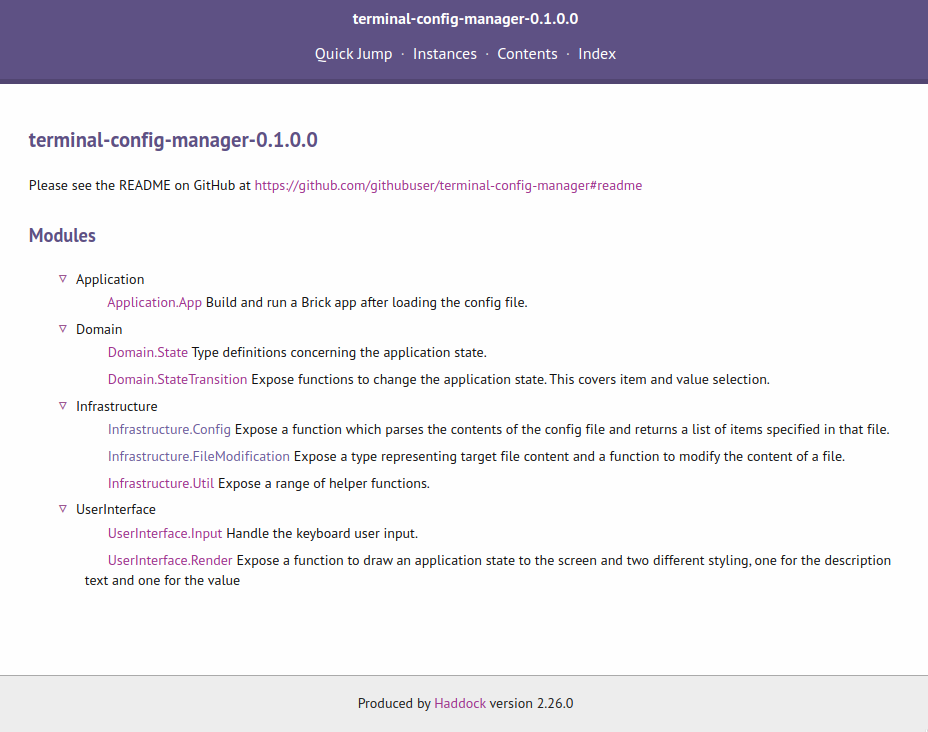
\includegraphics[scale=0.5]{module-documentation-index.png}}
\end{figure}

\begin{figure}[ht]
    \caption{Generierte Moduldokumentation, Domain.State}
    \label{module-doc-state}
    \fbox{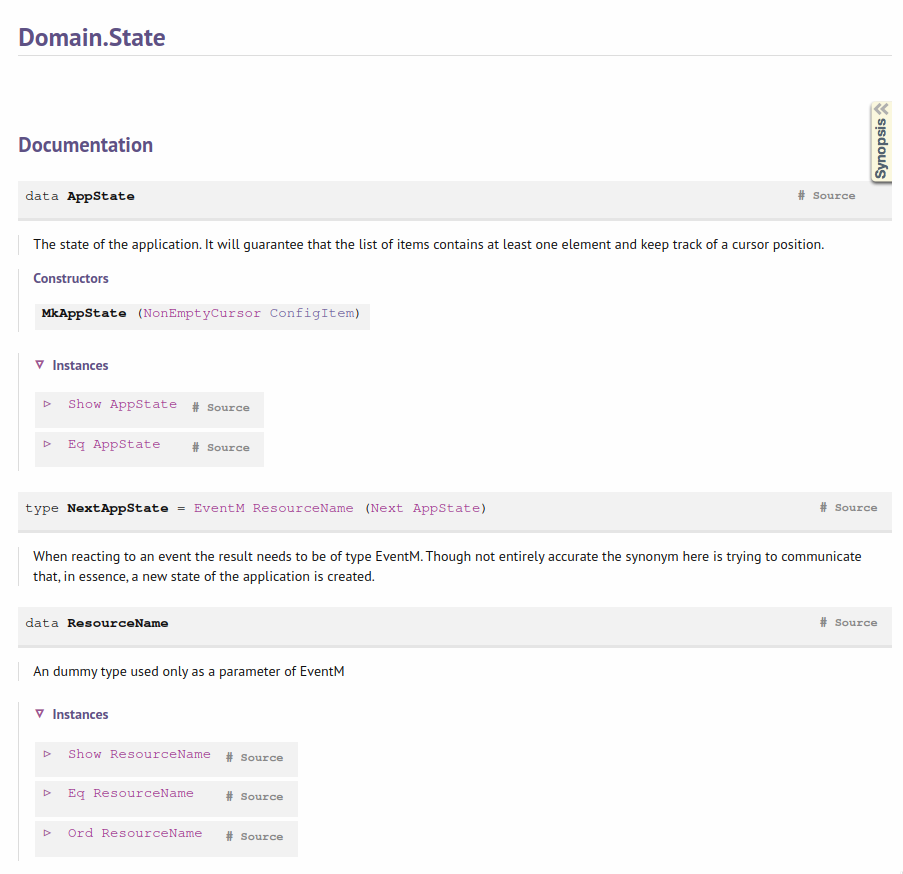
\includegraphics[scale=0.5]{module-documentation-state.png}}
\end{figure}

\begin{figure}[ht]
    \caption{Beispielschema für Modulabhängigkeiten beim Domain-Driven-Design \cite{domain-driven-design}}
    \label{domain-driven-design-layers}
    \centering\fbox{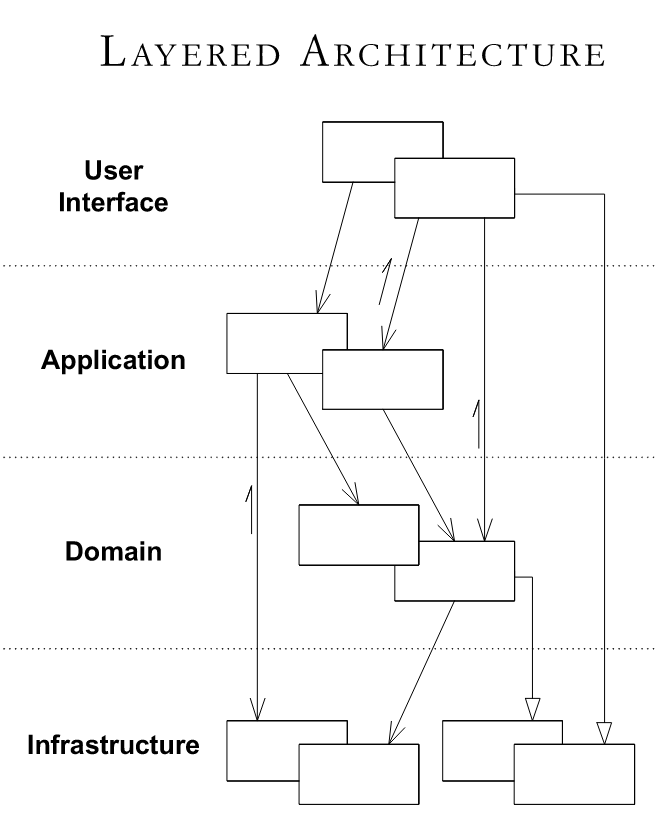
\includegraphics[scale=0.5]{domain-driven-design-layers.png}}
\end{figure}

\begin{figure}[ht]
    \caption{Graph der Modulabhängigkeiten}
    \label{module-dependency-graph}
    \centering\fbox{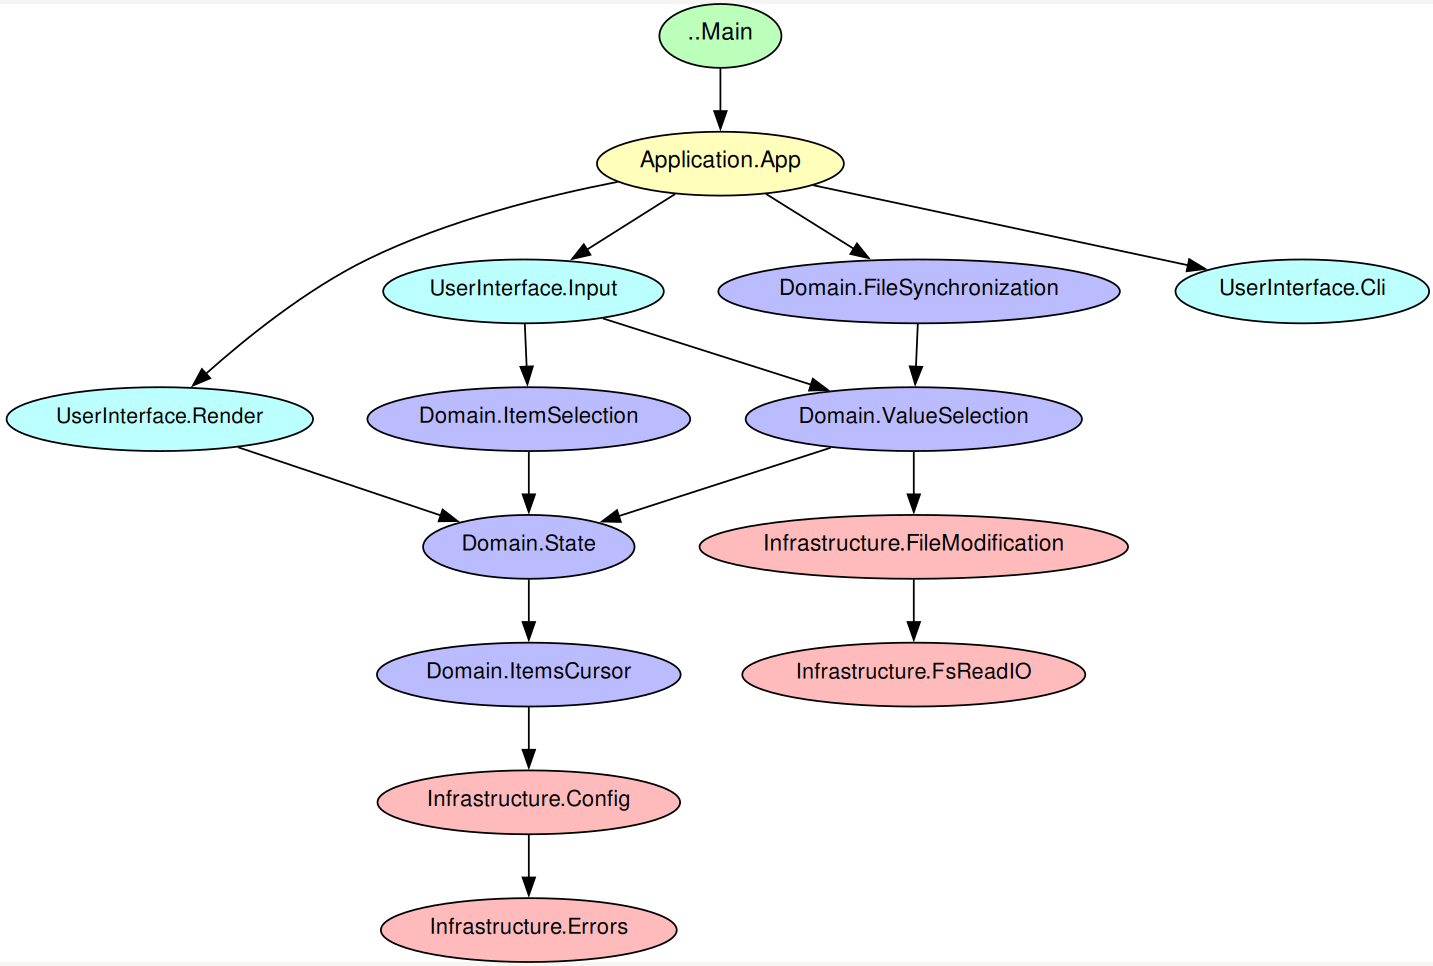
\includegraphics[scale=0.3]{module-dependency-graph.png}}
\end{figure}

\begin{figure}[ht]
    \caption{Ausgabe bei Ausführung der Testsuite}
    \label{test-suite}
    \centering\fbox{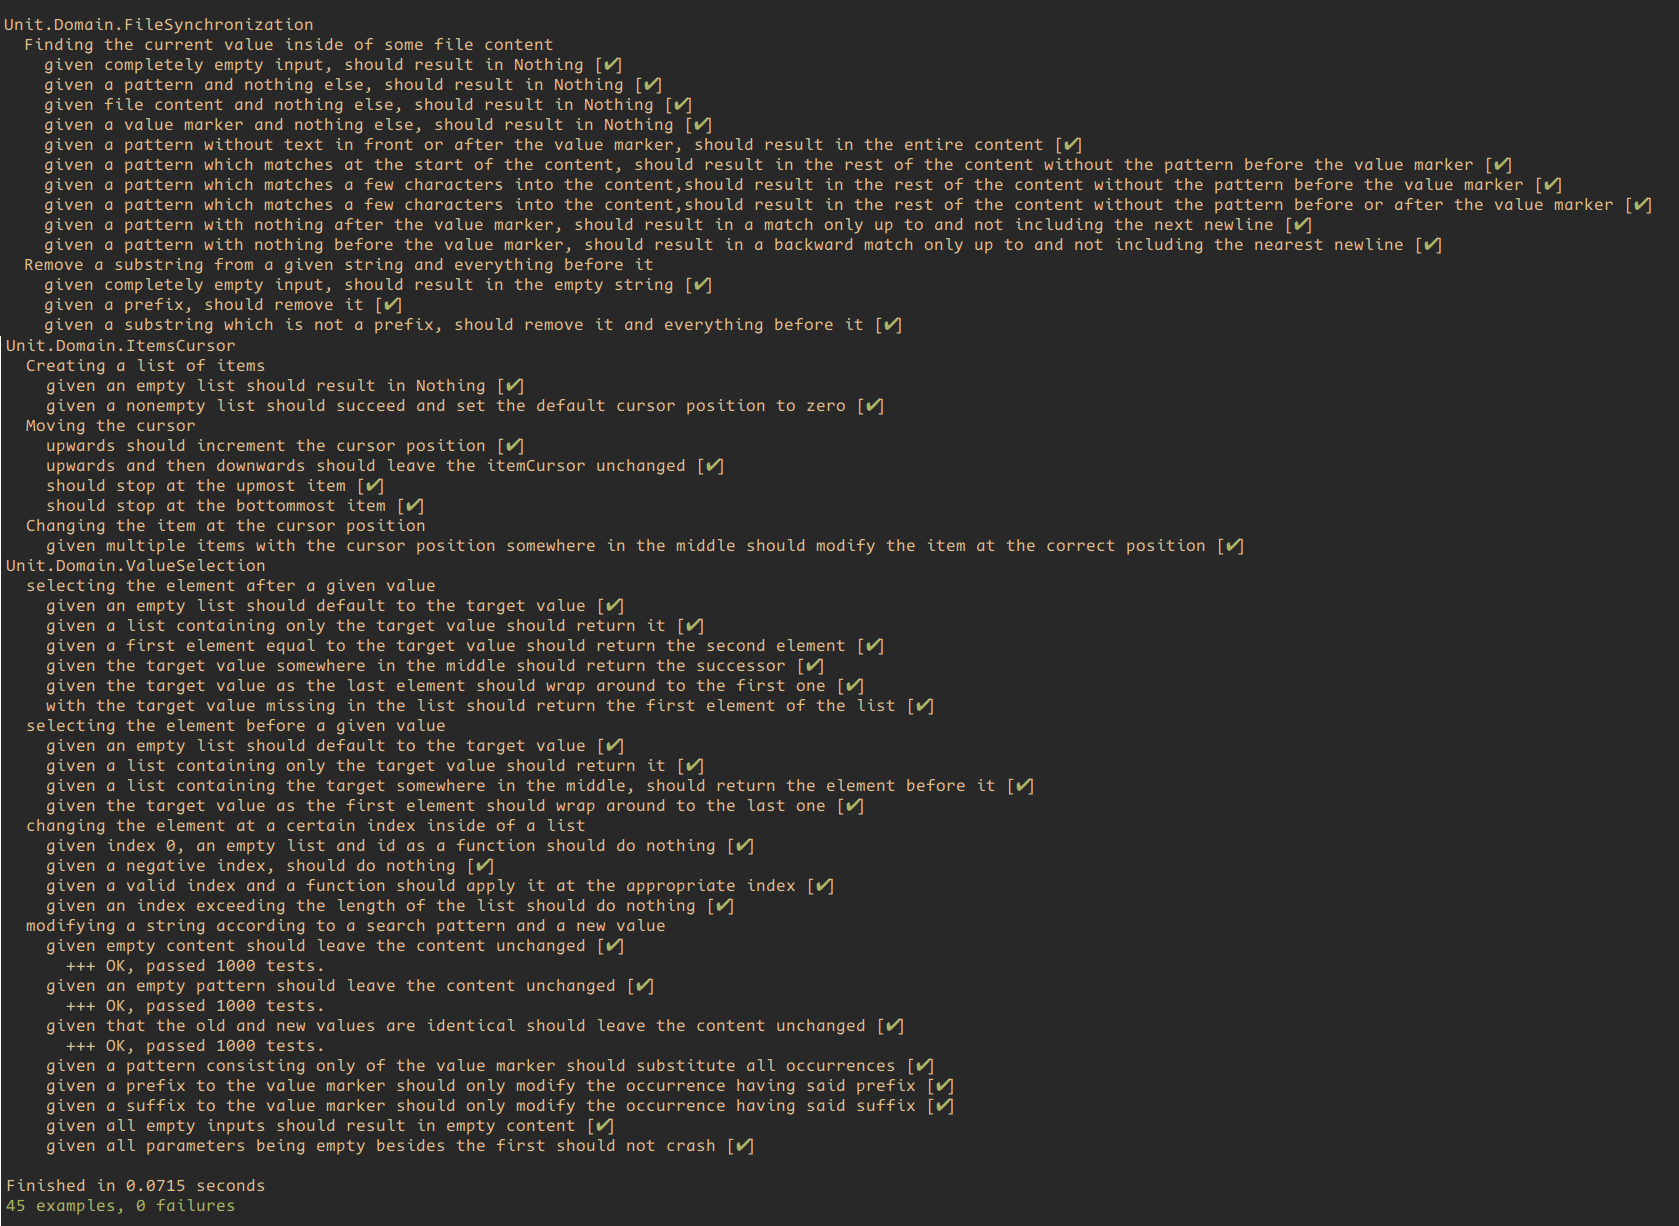
\includegraphics[scale=0.25]{full-test-suite.png}}
\end{figure}